\documentclass[11pt]{article}

\usepackage[margin=1in]{geometry}
\usepackage[T1]{fontenc}
\usepackage[utf8]{inputenc}
\usepackage{lmodern}
\usepackage{microtype}
\usepackage{amsmath,amssymb,amsthm,mathtools}
\usepackage{bm}
\usepackage{booktabs,array,longtable}
\usepackage{hyperref}
\usepackage{xcolor}
\usepackage[most]{tcolorbox}
\usepackage{tikz}
\usepackage{pgfplots}
\usepackage{pgfplotstable}
\usepackage{tikz-3dplot}
\usepackage{enumitem}
\usepackage{caption}
\usepackage{float}
\usepackage{fancyhdr}
\usepackage{titlesec}

\pgfplotsset{compat=1.18}
\usepgfplotslibrary{fillbetween}
\usetikzlibrary{arrows.meta,calc,intersections,patterns,decorations.pathreplacing,positioning,3d,backgrounds}

\hypersetup{
  colorlinks=true,
  linkcolor=blue!60!black,
  urlcolor=blue!60!black,
  citecolor=blue!60!black,
  pdftitle={Chapter 6. Functions of Several Variables}
}

\setlength{\headheight}{14pt}
\setlength{\parindent}{0pt}
\setlength{\parskip}{0.65em}
\setlist[itemize]{topsep=2pt,itemsep=2pt}
\setlist[enumerate]{topsep=2pt,itemsep=2pt}

\titleformat{\section}{\large\bfseries}{\thesection}{0.6em}{}
\titleformat{\subsection}{\normalsize\bfseries}{\thesubsection}{0.6em}{}

\pagestyle{fancy}
\fancyhf{}
\lhead{Chapter 6. Functions of Several Variables}
\rhead{\thepage}
\renewcommand{\headrulewidth}{0.4pt}

\newtcolorbox{chapteroverviewbox}{
  colback=blue!4,
  colframe=blue!50!black,
  boxrule=0.7pt,
  arc=2mm,
  left=2mm,right=2mm,top=1mm,bottom=1mm
}

\newtcolorbox{goalbox}{
  colback=green!4,
  colframe=green!45!black,
  title=Learning goals,
  fonttitle=\bfseries,
  boxrule=0.7pt,
  arc=2mm
}

\newtcolorbox{notebox}[1][]{
  colback=blue!3,
  colframe=blue!50!black,
  fonttitle=\bfseries,
  title=#1,
  boxrule=0.7pt,
  arc=2mm
}

\newtcolorbox{tipbox}[1][]{
  colback=green!3,
  colframe=green!45!black,
  fonttitle=\bfseries,
  title=#1,
  boxrule=0.7pt,
  arc=2mm
}

\newtcolorbox{warningbox}[1][]{
  colback=yellow!8,
  colframe=orange!75!black,
  fonttitle=\bfseries,
  title=#1,
  boxrule=0.7pt,
  arc=2mm
}

\newtcbtheorem[number within=section]{workedexample}{Worked example}{
  enhanced,
  breakable,
  colback=white,
  colframe=blue!60!black,
  colbacktitle=blue!60!black,
  fonttitle=\bfseries,
  boxrule=0.7pt,
  arc=1.5mm,
  left=2mm,right=2mm,top=1mm,bottom=1mm
}{ex}

\newcommand{\R}{\mathbb R}
\newcommand{\Range}{\operatorname{Range}}
\newcommand{\dd}{\,d}
\newcommand{\ds}{\displaystyle}

\begin{document}

\begin{center}
  {\LARGE\bfseries Chapter 6. Functions of Several Variables\par}
  \vspace{0.3em}
  {\large Scalar fields, domains, surfaces, level sets, and data landscapes\par}
\end{center}

\begin{chapteroverviewbox}
Single-variable calculus studies functions of the form $y=f(x)$, where one real input produces one real output. Multivariable calculus studies functions such as
\[
z=f(x,y), \qquad w=f(x,y,z), \qquad F=f(x_1,x_2,\ldots,x_n).
\]
The input is no longer a point on a line. It may be a point in the plane, a point in space, or a vector in a high-dimensional parameter space. The output is still a scalar: a height, temperature, density, probability, loss, likelihood, energy, cost, or risk.

This chapter develops the geometric language for these objects. We learn how to describe domains, draw surfaces, read contour maps, study level curves and level surfaces, and use lower-dimensional views to understand high-dimensional functions.
\end{chapteroverviewbox}

\begin{notebox}[Role in the book]
The next several chapters study limits, derivatives, gradients, optimization, and multiple integrals. All of those topics depend on the viewpoint developed here: a multivariable function is a scalar field over a region of space.
\end{notebox}

\begin{goalbox}
After studying this chapter, you should be able to:
\begin{enumerate}
  \item define functions of two, three, and $n$ variables;
  \item distinguish domain, codomain, and range;
  \item find domains defined by square roots, logarithms, denominators, and geometric restrictions;
  \item interpret the graph of $z=f(x,y)$ as a surface above a domain in the $xy$-plane;
  \item recognize planes, hemispheres, paraboloids, and saddle surfaces;
  \item compute and interpret level curves $f(x,y)=c$;
  \item interpret level surfaces $f(x,y,z)=c$;
  \item use slices, contour plots, heatmaps, and surface plots to visualize functions;
  \item connect multivariable functions to probability, statistics, optimization, data science, and machine learning.
\end{enumerate}
\end{goalbox}

\section{Functions of several variables}

A \emph{function of two variables} is a rule that assigns to each input pair $(x,y)$ in a domain $D\subseteq \R^2$ exactly one real number $f(x,y)$:
\[
f:D\subseteq \R^2\to \R.
\]
The set $D$ is the \emph{domain}. The set of all output values is the \emph{range}:
\[
\Range(f)=\{f(x,y):(x,y)\in D\}.
\]

A \emph{function of three variables} is a rule
\[
f:E\subseteq \R^3\to \R,\qquad (x,y,z)\mapsto f(x,y,z).
\]
More generally, a \emph{function of $n$ variables} is a rule
\[
f:D\subseteq \R^n\to \R,\qquad x=(x_1,x_2,\ldots,x_n)\mapsto f(x_1,x_2,\ldots,x_n).
\]
A function $f:\R^n\to\R$ is often called a \emph{scalar field} because it assigns a scalar value to each point in space.

\subsection*{Examples from science, statistics, and AI}

\begin{center}
\begin{tabular}{@{}>{\raggedright\arraybackslash}p{0.18\textwidth}p{0.18\textwidth}p{0.15\textwidth}p{0.34\textwidth}@{}}
\toprule
Function & Input & Output & Interpretation \\
\midrule
$T(x,y)$ & longitude and latitude & temperature & weather map \\
$p(x,y,z)$ & point in space & pressure & fluid or atmosphere \\
$\rho(x,y,z)$ & point in space & density & mass distribution \\
$L(\beta_0,\beta_1)$ & model parameters & squared error loss & linear regression \\
$\ell(\theta)$ & statistical parameter & log-likelihood & inference \\
$J(w_1,\ldots,w_n)$ & model weights & training objective & machine learning \\
\bottomrule
\end{tabular}
\end{center}

\begin{tipbox}[Modern viewpoint]
In data science and AI, the most important functions are often high-dimensional. A neural-network loss function may depend on millions or billions of parameters. We cannot draw its graph, but the ideas of domains, level sets, slices, gradients, and local approximations remain central.
\end{tipbox}

\section{Domains as regions}

Finding the domain is often the first step in studying a multivariable function. The algebraic restrictions are familiar from single-variable calculus, but now they describe regions in the plane or space.

\begin{center}
\begin{tabular}{@{}ll@{}}
\toprule
Expression & Restriction \\
\midrule
$\sqrt{g(x,y)}$ & $g(x,y)\ge 0$ \\
$\ln(g(x,y))$ & $g(x,y)>0$ \\
$\dfrac{1}{g(x,y)}$ & $g(x,y)\ne 0$ \\
$\arcsin(g(x,y))$ & $-1\le g(x,y)\le 1$ \\
\bottomrule
\end{tabular}
\end{center}

\begin{workedexample}{Square root and denominator}{sqrtden}
Find the domain of
\[
f(x,y)=\frac{\sqrt{y-x}}{y}.
\]
The square root requires $y-x\ge 0$, so $y\ge x$. The denominator requires $y\ne 0$. Therefore
\[
D=\{(x,y)\in \R^2:y\ge x,\; y\ne 0\}.
\]
This is the half-plane above the line $y=x$, with the portion of the line $y=0$ removed.
\end{workedexample}

\begin{workedexample}{Parabolic domain with excluded lines}{parabolicdomain}
Find the domain of
\[
g(x,y)=\frac{\sqrt{x^2-y}}{x^2-4}.
\]
The square root requires $x^2-y\ge 0$, so $y\le x^2$. The denominator requires $x^2-4\ne 0$, so $x\ne 2$ and $x\ne -2$. Thus
\[
D=\{(x,y)\in \R^2:y\le x^2,\; x\ne \pm 2\}.
\]
\end{workedexample}

\begin{figure}[H]
\centering
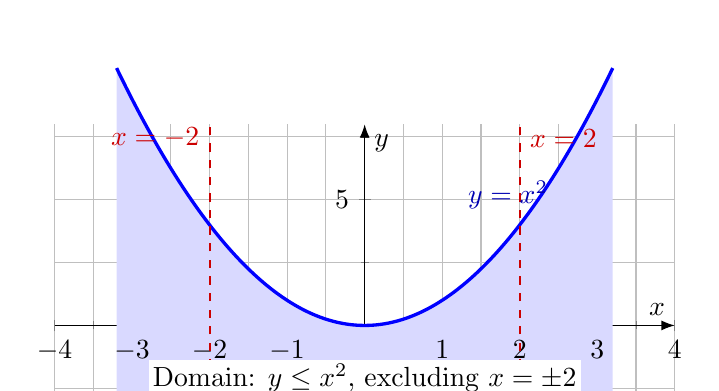
\begin{tikzpicture}
\begin{axis}[
  width=0.78\textwidth,
  height=0.42\textwidth,
  xmin=-4,xmax=4,
  ymin=-3,ymax=8,
  axis lines=middle,
  xlabel={$x$},ylabel={$y$},
  grid=both,
  minor tick num=1,
  axis line style={-Latex},
  samples=200,
  clip=false
]
\addplot[name path=parabola,domain=-3.2:3.2,very thick,blue] {x^2};
\path[name path=bottom] (axis cs:-3.2,-3) -- (axis cs:3.2,-3);
\addplot[blue!15] fill between[of=parabola and bottom,soft clip={domain=-3.2:3.2}];
\addplot[red!80!black,dashed,thick] coordinates {(2,-3) (2,8)} node[pos=0.95,right] {$x=2$};
\addplot[red!80!black,dashed,thick] coordinates {(-2,-3) (-2,8)} node[pos=0.95,left] {$x=-2$};
\node[blue!70!black] at (axis cs:1.85,5.2) {$y=x^2$};
\node[fill=white,inner sep=1.5pt] at (axis cs:0,-2.1) {Domain: $y\le x^2$, excluding $x=\pm 2$};
\end{axis}
\end{tikzpicture}
\caption{The domain of $\sqrt{x^2-y}/(x^2-4)$ is the region below the parabola $y=x^2$, with the vertical lines $x=\pm 2$ removed.}
\end{figure}

\begin{workedexample}{Logarithmic disk}{logdisk}
Find the domain of
\[
h(x,y)=\ln(9-x^2-y^2).
\]
The logarithm requires $9-x^2-y^2>0$, or equivalently,
\[
x^2+y^2<9.
\]
Thus the domain is the open disk of radius $3$ centered at the origin.
\end{workedexample}

\begin{figure}[H]
\centering
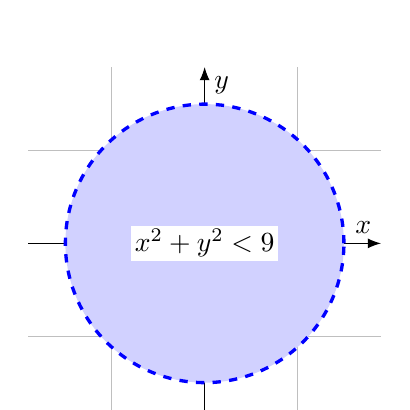
\begin{tikzpicture}
\begin{axis}[
  width=0.5\textwidth,
  height=0.5\textwidth,
  xmin=-3.8,xmax=3.8,
  ymin=-3.8,ymax=3.8,
  axis equal image,
  axis lines=middle,
  xlabel={$x$},ylabel={$y$},
  grid=both,
  axis line style={-Latex},
  clip=false
]
\addplot[draw=none,fill=blue!18,domain=0:360,samples=150] ({3*cos(x)},{3*sin(x)}) -- (axis cs:0,0) -- cycle;
\addplot[very thick,blue,dashed,domain=0:360,samples=200] ({3*cos(x)},{3*sin(x)});
\node[fill=white,inner sep=1.2pt] at (axis cs:0,0) {$x^2+y^2<9$};
\end{axis}
\end{tikzpicture}
\caption{The domain of $\ln(9-x^2-y^2)$ is the open disk $x^2+y^2<9$. The boundary circle is not included.}
\end{figure}

\begin{warningbox}[Common mistake]
For $\ln(9-x^2-y^2)$ the boundary circle $x^2+y^2=9$ is \emph{not} included, because $\ln(0)$ is undefined. For $\sqrt{9-x^2-y^2}$ the boundary is included, because $\sqrt{0}=0$.
\end{warningbox}

\section{Graphs of functions of two variables}

For a function $f:D\subseteq\R^2\to\R$, the \emph{graph} is the set of points in $\R^3$ given by
\[
\{(x,y,z):(x,y)\in D,\; z=f(x,y)\}.
\]
We usually write the graph as $z=f(x,y)$. The graph is a surface above or below the domain in the $xy$-plane.

\begin{workedexample}{A plane as a graph}{planegraph}
Let
\[
f(x,y)=6-2x-3y.
\]
Then
\[
z=6-2x-3y,
\]
or equivalently,
\[
2x+3y+z=6.
\]
This is a plane. It has $x$-intercept $3$, $y$-intercept $2$, and $z$-intercept $6$.
\end{workedexample}

\begin{figure}[H]
\centering
\tdplotsetmaincoords{68}{120}
\begin{tikzpicture}[tdplot_main_coords,scale=1.2]
  \coordinate (O) at (0,0,0);
  \coordinate (X) at (3.8,0,0);
  \coordinate (Y) at (0,2.8,0);
  \coordinate (Z) at (0,0,6.8);
  \coordinate (A) at (3,0,0);
  \coordinate (B) at (0,2,0);
  \coordinate (C) at (0,0,6);

  \filldraw[fill=blue!15,draw=blue!65!black,opacity=0.85] (A)--(B)--(C)--cycle;

  \draw[-Latex,thick] (O)--(X) node[below left] {$x$};
  \draw[-Latex,thick] (O)--(Y) node[below right] {$y$};
  \draw[-Latex,thick] (O)--(Z) node[right] {$z$};

  \draw[densely dashed] (A)--(C);
  \draw[densely dashed] (B)--(C);

  \fill (A) circle (1.2pt) node[below left] {$(3,0,0)$};
  \fill (B) circle (1.2pt) node[left] {$(0,2,0)$};
  \fill (C) circle (1.2pt) node[right] {$(0,0,6)$};
  \node[blue!60!black] at (1.4,0.9,3.2) {$2x+3y+z=6$};
\end{tikzpicture}
\caption{The graph of $f(x,y)=6-2x-3y$ is a plane. Its intercepts make the geometry transparent.}
\end{figure}

\begin{workedexample}{Upper hemisphere}{upperhemisphere}
Let
\[
f(x,y)=\sqrt{4-x^2-y^2}.
\]
The domain is determined by $4-x^2-y^2\ge 0$, so $x^2+y^2\le 4$. The graph satisfies
\[
z=\sqrt{4-x^2-y^2}.
\]
Squaring both sides gives
\[
x^2+y^2+z^2=4.
\]
Because $z\ge 0$, the graph is the upper hemisphere of radius $2$ centered at the origin. The range is $0\le z\le 2$.
\end{workedexample}

\begin{figure}[H]
\centering
\tdplotsetmaincoords{70}{120}
\begin{tikzpicture}[tdplot_main_coords,scale=1.55]
  \draw[-Latex,thick] (0,0,0)--(2.8,0,0) node[below left] {$x$};
  \draw[-Latex,thick] (0,0,0)--(0,2.8,0) node[below right] {$y$};
  \draw[-Latex,thick] (0,0,0)--(0,0,2.8) node[right] {$z$};
  \shade[ball color=blue!18,opacity=0.9] (0,0,1.05) circle (1.75cm);
  \draw[thick,blue!70!black] (0,0,1.05) circle (1.75cm);
  \draw[thick,blue!70!black] (-1.75,0,1.05) arc[start angle=180,end angle=360,x radius=1.75cm,y radius=0.55cm];
  \draw[dashed,blue!70!black] (-1.75,0,1.05) arc[start angle=180,end angle=0,x radius=1.75cm,y radius=0.55cm];
  \draw[dashed] (0,0,0) circle (1.75cm);
  \node[fill=white,inner sep=1.2pt] at (0.15,1.55,2.1) {$x^2+y^2+z^2=4$, $z\ge 0$};
\end{tikzpicture}
\caption{The graph of $f(x,y)=\sqrt{4-x^2-y^2}$ is the upper hemisphere of radius $2$.}
\end{figure}

\begin{workedexample}{Elliptic paraboloid}{ellipticparaboloid}
Let
\[
f(x,y)=x^2+9y^2.
\]
The domain is all of $\R^2$. Since squares are nonnegative, the range is $z\ge 0$. The graph
\[
z=x^2+9y^2
\]
is an \emph{elliptic paraboloid}. It opens upward, and it rises faster in the $y$-direction than in the $x$-direction because the coefficient of $y^2$ is larger.
\end{workedexample}

\begin{workedexample}{A saddle surface}{saddlegraph}
Let
\[
f(x,y)=x^2-y^2.
\]
The graph
\[
z=x^2-y^2
\]
is a saddle surface. Along the $x$-axis, where $y=0$, it becomes $z=x^2$, which opens upward. Along the $y$-axis, where $x=0$, it becomes $z=-y^2$, which opens downward.
\end{workedexample}

\begin{figure}[H]
\centering
\begin{minipage}{0.49\textwidth}
\centering
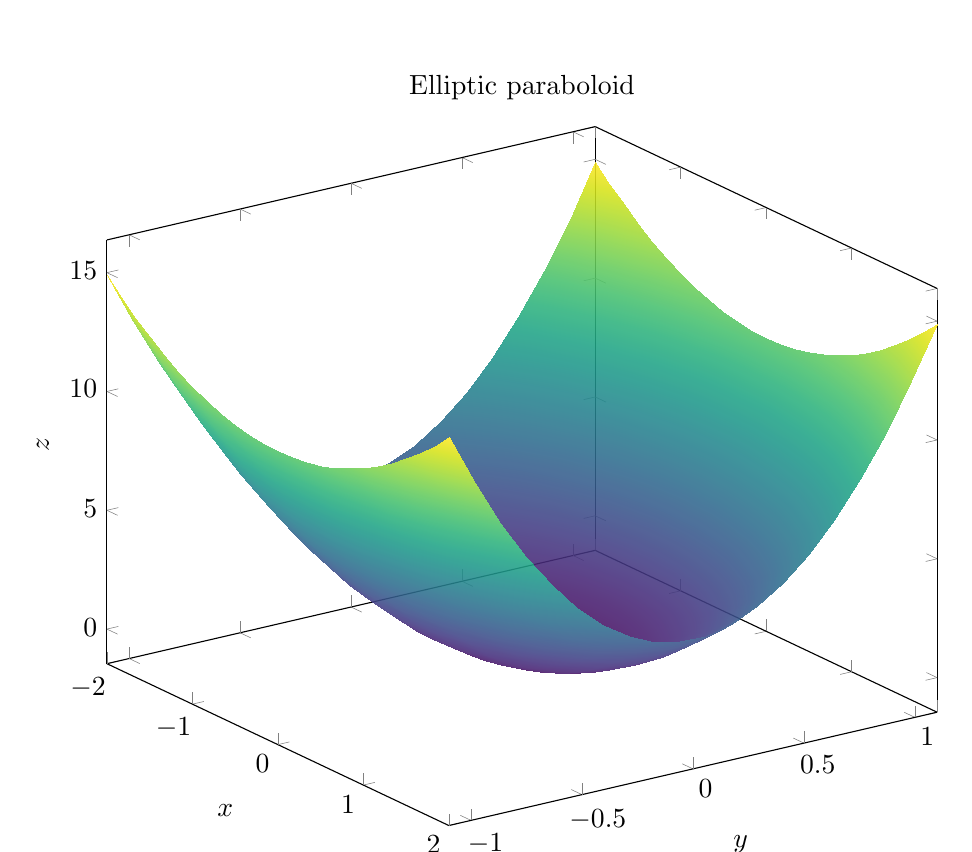
\begin{tikzpicture}
\begin{axis}[
  width=\textwidth,
  view={55}{25},
  xlabel={$x$},ylabel={$y$},zlabel={$z$},
  domain=-2:2, y domain=-1.1:1.1,
  samples=25,samples y=20,
  colormap/viridis,
  title={Elliptic paraboloid},
]
\addplot3[surf,shader=interp,opacity=0.88] {x^2 + 9*y^2};
\end{axis}
\end{tikzpicture}
\end{minipage}
\hfill
\begin{minipage}{0.49\textwidth}
\centering
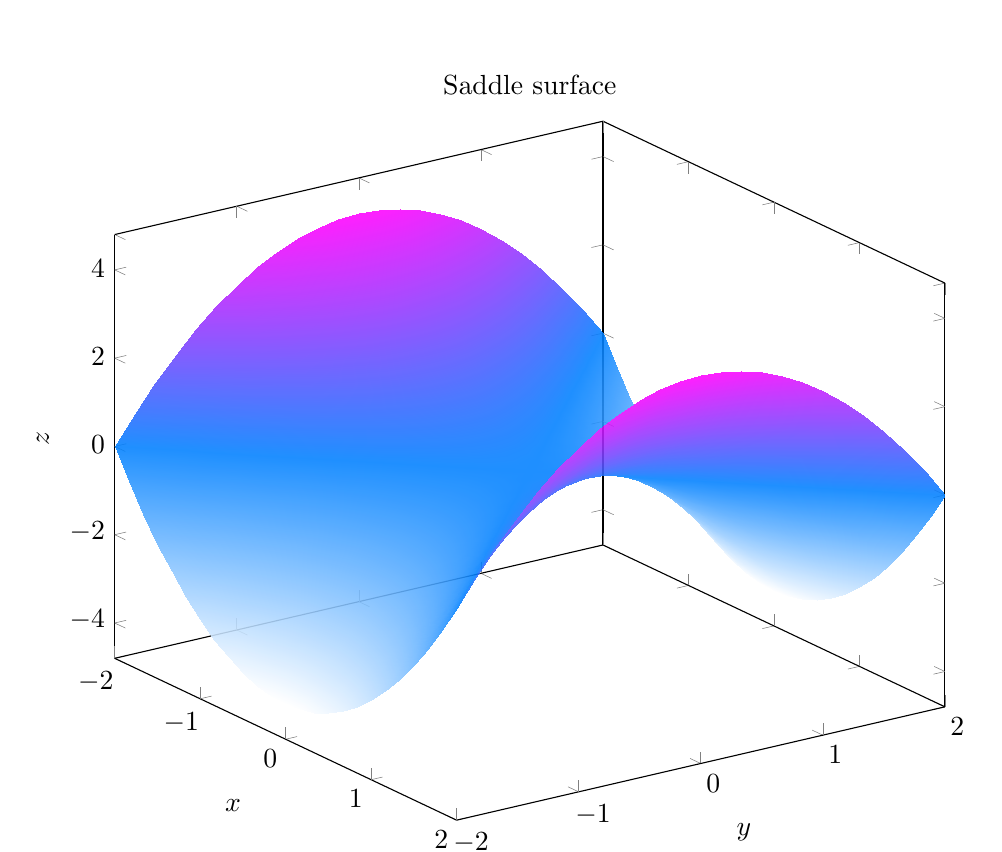
\begin{tikzpicture}
\begin{axis}[
  width=\textwidth,
  view={55}{25},
  xlabel={$x$},ylabel={$y$},zlabel={$z$},
  domain=-2:2, y domain=-2:2,
  samples=25,samples y=25,
  colormap/cool,
  title={Saddle surface},
]
\addplot3[surf,shader=interp,opacity=0.88] {x^2 - y^2};
\end{axis}
\end{tikzpicture}
\end{minipage}
\caption{Two basic surfaces: the elliptic paraboloid $z=x^2+9y^2$ and the saddle surface $z=x^2-y^2$.}
\end{figure}

\section{Slices and traces}

A surface can be understood by taking lower-dimensional slices. For $z=f(x,y)$:
\begin{itemize}
  \item fixing $y=y_0$ gives the curve $z=f(x,y_0)$ in a vertical plane parallel to the $xz$-plane;
  \item fixing $x=x_0$ gives the curve $z=f(x_0,y)$ in a vertical plane parallel to the $yz$-plane;
  \item fixing $z=c$ gives the level curve $f(x,y)=c$ in the $xy$-plane.
\end{itemize}
Slices connect single-variable calculus to multivariable calculus. Partial derivatives in later chapters measure slopes of coordinate slices.

\begin{workedexample}{Slices of an elliptic paraboloid}{slices}
For
\[
z=x^2+9y^2,
\]
fixing $y=0$ gives $z=x^2$, while fixing $x=0$ gives $z=9y^2$. The second slice is steeper.
\end{workedexample}

\begin{figure}[H]
\centering
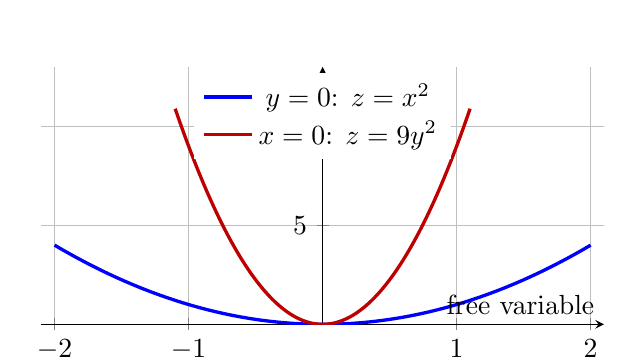
\begin{tikzpicture}
\begin{axis}[
  width=0.72\textwidth,
  height=0.4\textwidth,
  xmin=-2.1,xmax=2.1,
  ymin=0,ymax=13,
  axis lines=middle,
  xlabel={free variable},
  ylabel={$z$},
  grid=both,
  legend style={at={(0.5,0.98)},anchor=north,fill=white,draw=none}
]
\addplot[very thick,blue,domain=-2:2,samples=150] {x^2};
\addlegendentry{$y=0$: $z=x^2$}
\addplot[very thick,red!75!black,domain=-1.1:1.1,samples=150] {9*x^2};
\addlegendentry{$x=0$: $z=9y^2$}
\end{axis}
\end{tikzpicture}
\caption{Coordinate slices of $z=x^2+9y^2$ show different rates of change in the $x$ and $y$ directions.}
\end{figure}

\section{Level curves and contour maps}

A \emph{level curve} of a function $f(x,y)$ is a curve of the form
\[
f(x,y)=c,
\]
where $c$ is a constant in the range of $f$.

Geometrically, the level curve $f(x,y)=c$ is obtained by intersecting the surface $z=f(x,y)$ with the horizontal plane $z=c$ and projecting the intersection down to the $xy$-plane. Contour maps are collections of level curves.

\begin{tipbox}[How to read contours]
Where level curves are close together, the function changes rapidly. Where level curves are far apart, the function changes slowly.
\end{tipbox}

\begin{workedexample}{Circular level curves}{circularlevels}
Let
\[
f(x,y)=x^2+y^2.
\]
The level curve $f(x,y)=c$ is
\[
x^2+y^2=c.
\]
For $c>0$, this is a circle centered at the origin with radius $\sqrt{c}$.
\end{workedexample}

\begin{workedexample}{Elliptic level curves}{ellipticlevels}
Let
\[
f(x,y)=x^2+9y^2.
\]
The level curve $f(x,y)=c$ is
\[
x^2+9y^2=c.
\]
For $c>0$, these are ellipses.
\end{workedexample}

\begin{figure}[H]
\centering
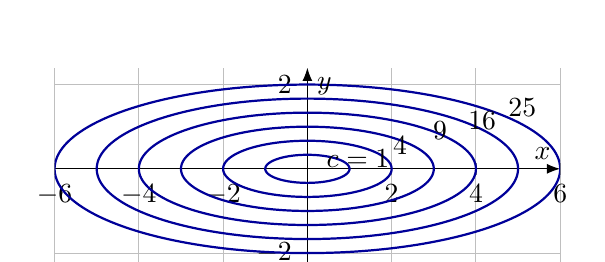
\begin{tikzpicture}
\begin{axis}[
  width=0.66\textwidth,
  height=0.42\textwidth,
  xmin=-6,xmax=6,
  ymin=-2.4,ymax=2.4,
  axis equal image,
  axis lines=middle,
  xlabel={$x$},ylabel={$y$},
  grid=both,
  axis line style={-Latex}
]
\foreach \c in {1,4,9,16,25,36}{
  \addplot[domain=0:360,samples=220,blue!60!black,thick] ({sqrt(\c)*cos(x)},{sqrt(\c)/3*sin(x)});
}
\node at (axis cs:1.2,0.25) {$c=1$};
\node at (axis cs:2.2,0.55) {$4$};
\node at (axis cs:3.15,0.9) {$9$};
\node at (axis cs:4.15,1.15) {$16$};
\node at (axis cs:5.1,1.45) {$25$};
\end{axis}
\end{tikzpicture}
\caption{Level curves of $f(x,y)=x^2+9y^2$ are ellipses. Larger level values produce larger ellipses.}
\end{figure}

\begin{workedexample}{Exponential level curves}{explevels}
Let
\[
f(x,y)=xe^{4y}.
\]
A level curve $f(x,y)=c$ satisfies
\[
xe^{4y}=c.
\]
If $x\ne 0$ and $c/x>0$, then
\[
y=\frac14\ln\!\left(\frac{c}{x}\right).
\]
This shows that level curves need not be lines, circles, parabolas, or ellipses.
\end{workedexample}

\section{Heatmaps and data surfaces}

A multivariable function may be known through data rather than a formula. For example, a temperature field may be measured on a grid of locations, or a loss function may be evaluated at many parameter values.

A \emph{heatmap} colors the plane according to function values. A \emph{contour plot} draws level curves. Both are useful when a full surface plot is difficult to read.

\section{Functions of three variables and level surfaces}

A function of three variables has the form $f(x,y,z)$. Its graph would be $w=f(x,y,z)$, which lives in four-dimensional space. Since we cannot directly draw a four-dimensional graph, we usually study \emph{level surfaces}:
\[
f(x,y,z)=c.
\]

\begin{workedexample}{Spherical level surfaces}{spherelevels}
Let
\[
f(x,y,z)=x^2+y^2+z^2.
\]
The level surface $f(x,y,z)=c$ is
\[
x^2+y^2+z^2=c.
\]
For $c>0$, this is a sphere of radius $\sqrt c$ centered at the origin.
\end{workedexample}

\begin{figure}[H]
\centering
\tdplotsetmaincoords{70}{120}
\begin{tikzpicture}[tdplot_main_coords,scale=1.5]
  \draw[-Latex,thick] (0,0,0)--(2.8,0,0) node[below left] {$x$};
  \draw[-Latex,thick] (0,0,0)--(0,2.8,0) node[below right] {$y$};
  \draw[-Latex,thick] (0,0,0)--(0,0,2.8) node[right] {$z$};
  \shade[ball color=blue!20,opacity=0.95] (0,0,0) circle (1.75cm);
  \draw[thick,blue!70!black] (0,0,0) circle (1.75cm);
  \draw[dashed,blue!70!black] (-1.75,0,0) arc[start angle=180,end angle=0,x radius=1.75cm,y radius=0.55cm];
  \draw[thick,blue!70!black] (-1.75,0,0) arc[start angle=180,end angle=360,x radius=1.75cm,y radius=0.55cm];
  \node[fill=white,inner sep=1.2pt] at (0.15,1.7,1.7) {$x^2+y^2+z^2=4$};
\end{tikzpicture}
\caption{A level surface of $f(x,y,z)=x^2+y^2+z^2$ is a sphere.}
\end{figure}

\begin{workedexample}{Plane level surfaces}{planelevels}
Let
\[
f(x,y,z)=2x-y+3z.
\]
The level surface $f(x,y,z)=c$ is
\[
2x-y+3z=c.
\]
For each value of $c$, this is a plane. Different values of $c$ give parallel planes.
\end{workedexample}

\begin{workedexample}{Ellipsoid level surfaces}{ellipsoidlevels}
Let
\[
f(x,y,z)=\frac{x^2}{4}+\frac{y^2}{9}+z^2.
\]
The level surface $f(x,y,z)=1$ is
\[
\frac{x^2}{4}+\frac{y^2}{9}+z^2=1,
\]
an ellipsoid with semi-axis lengths $2$, $3$, and $1$.
\end{workedexample}

\section{Functions on high-dimensional spaces}

In statistics and machine learning, a function often has many variables. Suppose a regression model predicts
\[
\widehat y_i=\beta_0+\beta_1x_i.
\]
The least-squares loss is
\[
L(\beta_0,\beta_1)=\sum_{i=1}^m \left(y_i-(\beta_0+\beta_1x_i)\right)^2.
\]
This is a function $L:\R^2\to\R$. For a model with $p$ predictors, the parameter vector is
\[
\beta=(\beta_0,\beta_1,\ldots,\beta_p),
\]
and the loss becomes a function $L:\R^{p+1}\to\R$.

We cannot draw this graph when $p$ is large, but we can still study slices, contours, gradients, and local quadratic approximations.

\begin{figure}[H]
\centering
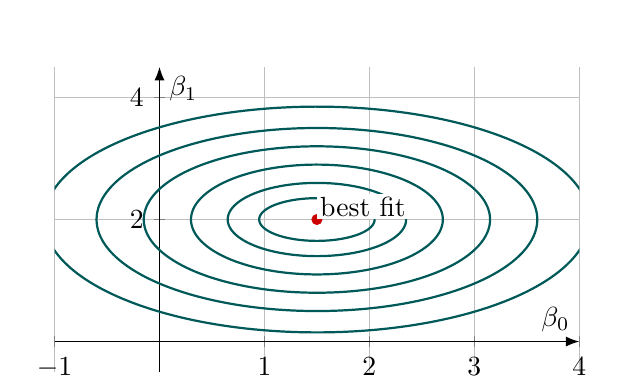
\begin{tikzpicture}
\begin{axis}[
  width=0.68\textwidth,
  height=0.45\textwidth,
  xmin=-1,xmax=4,
  ymin=-0.5,ymax=4.5,
  axis lines=middle,
  xlabel={$\beta_0$},ylabel={$\beta_1$},
  grid=both,
  axis line style={-Latex}
]
\foreach \a/\b in {0.55/0.35,0.85/0.6,1.2/0.9,1.65/1.2,2.1/1.5,2.6/1.85}{
  \addplot[domain=0:360,samples=220,teal!70!black,thick] ({1.5 + \a*cos(x)},{2.0 + \b*sin(x)});
}
\fill[red!80!black] (axis cs:1.5,2.0) circle (2pt);
\node[above right,fill=white,inner sep=1pt] at (axis cs:1.5,2.0) {best fit};
\end{axis}
\end{tikzpicture}
\caption{A two-parameter least-squares loss landscape. Smaller contours indicate lower loss.}
\end{figure}

\subsection*{Likelihood functions}
In statistics, a likelihood function assigns to each parameter value a number measuring how compatible that parameter is with the observed data. For example, for a normal model with known variance, the log-likelihood has the form
\[
\ell(\mu)=-\frac{1}{2\sigma^2}\sum_{i=1}^m (x_i-\mu)^2+\text{constant}.
\]
For a multivariate model, $\theta$ may have many components, and the log-likelihood becomes
\[
\ell(\theta):\R^n\to\R.
\]
Thus optimization in statistics is also multivariable calculus.

\section{Representations of a multivariable function}

\begin{center}
\begin{tabular}{@{}>{\raggedright\arraybackslash}p{0.16\textwidth}>{\raggedright\arraybackslash}p{0.29\textwidth}>{\raggedright\arraybackslash}p{0.33\textwidth}@{}}
\toprule
Representation & Meaning & Example \\
\midrule
Verbal & description in words & temperature depends on longitude and latitude \\
Algebraic & formula & $f(x,y)=x^2+9y^2$ \\
Numerical & table or data grid & measured temperatures on a map \\
Visual & surface, contour, heatmap & graph of $z=f(x,y)$ \\
Algorithmic & code that computes values & simulation or machine learning model \\
\bottomrule
\end{tabular}
\end{center}

Modern applied mathematics often moves among all five. Data are numerical, models are algebraic or algorithmic, and interpretation requires visual and verbal reasoning.

\section{Common surfaces and level sets}

\begin{center}
\begin{tabular}{@{}lll@{}}
\toprule
Equation & Shape & Key feature \\
\midrule
$z=ax+by+c$ & plane & linear surface \\
$z=x^2+y^2$ & circular paraboloid & opens upward \\
$z=x^2+9y^2$ & elliptic paraboloid & different curvature in different directions \\
$z=x^2-y^2$ & saddle & rises in one direction, falls in another \\
$x^2+y^2+z^2=r^2$ & sphere & level surface of distance squared \\
$x^2+y^2=r^2$ & cylinder & no restriction on $z$ \\
$z=\sqrt{r^2-x^2-y^2}$ & upper hemisphere & graph over a disk \\
$\dfrac{x^2}{a^2}+\dfrac{y^2}{b^2}+\dfrac{z^2}{c^2}=1$ & ellipsoid & stretched sphere \\
\bottomrule
\end{tabular}
\end{center}

Recognizing these shapes will help with optimization, multiple integration, and vector calculus.

\section{Worked synthesis: one function, many views}

Consider
\[
f(x,y)=e^{-x^2-y^2}.
\]

\textbf{Domain.} The exponential function is defined for every real number, so the domain is all of $\R^2$.

\textbf{Range.} Since $x^2+y^2\ge 0$, we have $-x^2-y^2\le 0$, so
\[
0<f(x,y)\le 1.
\]
The maximum value is $1$ at $(0,0)$.

\textbf{Graph.} The graph is a bell-shaped surface centered at the origin.

\textbf{Level curves.} A level curve satisfies
\[
e^{-x^2-y^2}=c.
\]
For $0<c\le 1$, taking natural logarithms gives
\[
x^2+y^2=-\ln c.
\]
Thus the level curves are circles centered at the origin.

\begin{figure}[H]
\centering
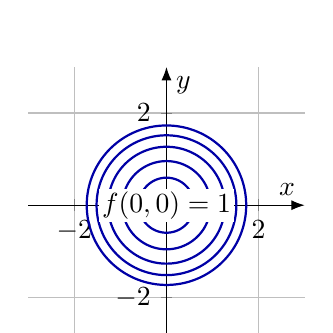
\begin{tikzpicture}
\begin{axis}[
  width=0.66\textwidth,
  height=0.42\textwidth,
  xmin=-3,xmax=3,
  ymin=-3,ymax=3,
  axis equal image,
  axis lines=middle,
  xlabel={$x$},ylabel={$y$},
  grid=both,
  axis line style={-Latex}
]
\foreach \c in {0.05,0.1,0.2,0.4,0.7,0.9}{
  \pgfmathsetmacro{\rad}{sqrt(-ln(\c))}
  \addplot[domain=0:360,samples=220,blue!65!black,thick] ({\rad*cos(x)},{\rad*sin(x)});
}
\node[fill=white,inner sep=1pt] at (axis cs:0,0) {$f(0,0)=1$};
\end{axis}
\end{tikzpicture}
\caption{The function $e^{-x^2-y^2}$ has circular level curves, reflecting its radial symmetry.}
\end{figure}

This example is a first glimpse of the geometry behind multivariate normal densities, radial basis functions, kernel methods, and smooth energy landscapes.

\section{Common mistakes}

\begin{warningbox}[Mistake 1: Confusing graph and domain]
The domain of $f(x,y)$ is a region in the $xy$-plane. The graph of $f$ is a surface in $xyz$-space. For example, the domain of $\sqrt{4-x^2-y^2}$ is a disk, while the graph is a hemisphere.
\end{warningbox}

\begin{warningbox}[Mistake 2: Forgetting strict inequalities]
For logarithms, the input must be positive, not merely nonnegative. Thus $\ln(4-x^2-y^2)$ has domain $x^2+y^2<4$, not $x^2+y^2\le 4$.
\end{warningbox}

\begin{warningbox}[Mistake 3: Thinking all level curves are circles]
Level curves may be lines, ellipses, hyperbolas, logarithmic curves, or more complicated curves. Their shape depends on the function.
\end{warningbox}

\section{Practice problems}

\begin{enumerate}
  \item Find and sketch the domain of $f(x,y)=\sqrt{x+y}$.
  \item Find and sketch the domain of $f(x,y)=\sqrt{x+y}/(x-y)$.
  \item Find and sketch the domain of $f(x,y)=\ln(4-x^2-y^2)$.
  \item Find the domain and range of $f(x,y)=\sqrt{9-x^2-y^2}$.
  \item Describe the graph of $z=3x-2y+5$.
  \item Describe the graph of $z=x^2+4y^2$.
  \item Describe the graph of $z=x^2-y^2$.
  \item Find the level curves of $f(x,y)=x^2+y^2$.
  \item Find the level curves of $f(x,y)=x^2+4y^2$.
  \item Find the level curves of $f(x,y)=xy$.
  \item Find the level curve of $f(x,y)=e^{-x^2-y^2}$ corresponding to $c=1/2$.
  \item Find the level surface of $f(x,y,z)=x^2+y^2+z^2$ through the point $(1,2,2)$.
  \item Describe the level surfaces of $f(x,y,z)=x+y+z$.
  \item Describe the level surface $x^2/4+y^2/9+z^2=1$.
  \item Give an example of a function $L:\R^n\to\R$ that appears in statistics, machine learning, economics, physics, or engineering.
\end{enumerate}

\section{Applied and computational exercises}

\begin{enumerate}
  \item Plot the surface $z=\sin x\cos y$ on $[-2\pi,2\pi]\times[-2\pi,2\pi]$.
  \item Draw contour plots for $f(x,y)=x^2-y^2$.
  \item Generate a grid of values for $f(x,y)=e^{-x^2-y^2}$ and display it as a heatmap.
  \item For $f(x,y)=x^2+4y^2$, compare the contours for levels $1$, $4$, $9$, and $16$.
  \item Simulate noisy data from a line $y=\beta_0+\beta_1x+\varepsilon$ and plot the loss contours in the $(\beta_0,\beta_1)$-plane.
  \item Choose a function of three variables and describe at least three of its level surfaces.
\end{enumerate}

\section{Chapter summary}

A function of several variables assigns one scalar output to each input point in a multidimensional domain:
\[
f:D\subseteq\R^n\to\R.
\]
The main ideas of this chapter are:
\begin{itemize}
  \item domains of multivariable functions are regions in $\R^n$;
  \item the graph of $z=f(x,y)$ is a surface in $\R^3$;
  \item level curves $f(x,y)=c$ show where a two-variable function is constant;
  \item level surfaces $f(x,y,z)=c$ play the same role for functions of three variables;
  \item slices and traces reduce multivariable functions to single-variable views;
  \item high-dimensional functions in statistics and AI are studied through contours, slices, heatmaps, gradients, and optimization paths.
\end{itemize}

In the next chapter, we study limits and continuity. The key new issue is that points can approach a target point from infinitely many directions.

\end{document}
